\documentclass[dvisvgm,tikz]{standalone}
\begin{document}
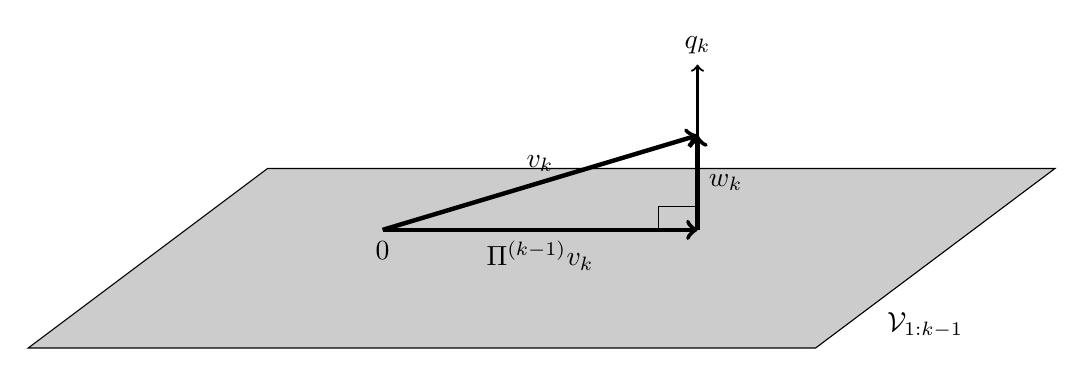
\begin{tikzpicture}
    \begin{scope}[xscale=5,yscale=3]
      \draw[xslant=0.8,fill=black!20] (-0.5,-0.5) rectangle (1.5,0.26);
      \draw[ultra thick,->]
        (0,0) node[below] {$0$} --
        (0.8,0) node[midway,below] {$\Pi^{(k-1)} v_k$};
      \node[above left] at (1.5,-0.5) {$\mathcal{V}_{1:k-1}$};
    \end{scope}
    \begin{scope}[xscale=5,yscale=3]
    \draw[ultra thick,->]
      (0,0) -- (0.8,0.4) node[above,midway] {$v_k$};
    \draw[ultra thick,->]
      (0.8,0) -- (0.8,0.4) node[midway,right] {$w_k$};
    \draw[thick,->]
      (0.8,0) -- (0.8,0.7) node[above] {$q_k$};
    \draw (0.7,0) -- (0.7,0.1) -- (0.8,0.1);
    \end{scope}
\end{tikzpicture}
\end{document}
